\documentclass[tikz,border=10pt]{standalone}
\usepackage{amsmath,amssymb}
\usepackage{newpxtext,newpxmath}
\usepackage{pgfplots}
\pgfplotsset{compat=1.18}
\usetikzlibrary{arrows.meta}

\definecolor{inkDark}{HTML}{1E293B}
\definecolor{slateSub}{HTML}{334155}
\definecolor{pathBlue}{HTML}{005A9C}
\definecolor{accentRed}{HTML}{B91C1C}
\definecolor{accentTeal}{HTML}{0E6251}
\definecolor{accentAmber}{HTML}{B45309}
\definecolor{bandBlue}{HTML}{DBEAFE}
\definecolor{boxFill}{HTML}{F8FAFC}

\begin{document}
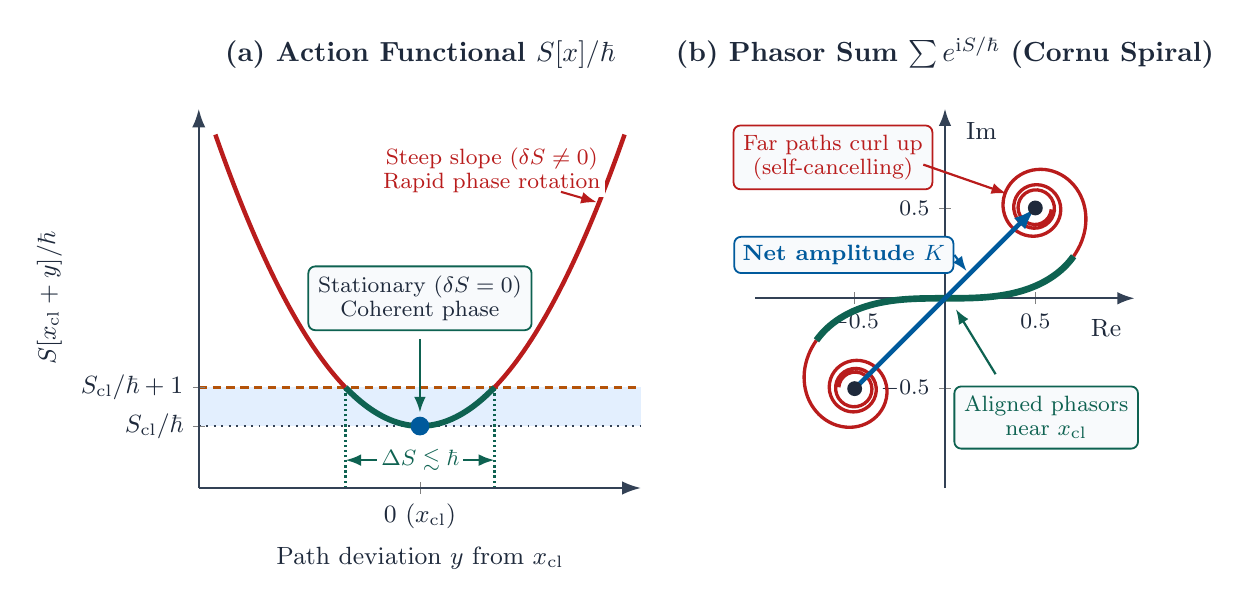
\begin{tikzpicture}[every node/.style={text=inkDark}]

    % =========================================================
    % Panel (a): Action functional S[x]/hbar across path space
    % =========================================================
    \begin{axis}[
        name=axA,
        width=7.2cm,
        height=6.4cm,
        title={(a) Action Functional $S[x]/\hbar$},
        title style={font=\bfseries\normalsize, text=inkDark, yshift=5pt},
        xmin=-4.0, xmax=4.0,
        ymin=0.0, ymax=9.8,
        axis lines=left,
        axis on top,
        axis line style={-{Latex[length=2.4mm,width=1.7mm]}, line width=0.9pt, draw=slateSub},
        xlabel={Path deviation $y$ from $x_{\mathrm{cl}}$},
        ylabel={$S[x_{\mathrm{cl}} + y] / \hbar$},
        xlabel style={font=\small, text=inkDark},
        ylabel style={font=\small, text=inkDark},
        xtick={0},
        xticklabels={$0$ ($x_{\mathrm{cl}}$)},
        ytick={1.6, 2.6},
        yticklabels={$S_{\mathrm{cl}}/\hbar$, $S_{\mathrm{cl}}/\hbar + 1$},
        tick label style={font=\small, text=inkDark}
    ]
        % Horizontal band Delta S <= hbar
        \fill[bandBlue, opacity=0.78] (axis cs:-4.0, 1.6) rectangle (axis cs:4.0, 2.6);
        \draw[accentAmber, line width=0.85pt, densely dashed] (axis cs:-4.0, 2.6) -- (axis cs:4.0, 2.6);
        \draw[slateSub, line width=0.7pt, dotted] (axis cs:-4.0, 1.6) -- (axis cs:4.0, 1.6);

        % Vertical corridor bounds where 0.55*u^2 = 1 => |u| = 1.348
        \draw[accentTeal, line width=0.85pt, densely dotted] (axis cs:-1.348, 0) -- (axis cs:-1.348, 2.6);
        \draw[accentTeal, line width=0.85pt, densely dotted] (axis cs: 1.348, 0) -- (axis cs: 1.348, 2.6);

        % Action parabola: far regions in red, stationary bottom in teal
        \addplot[domain=-3.7:-1.348, samples=60, line width=1.6pt, draw=accentRed] {1.6 + 0.55*x*x};
        \addplot[domain= 1.348: 3.7, samples=60, line width=1.6pt, draw=accentRed] {1.6 + 0.55*x*x};
        \addplot[domain=-1.348:1.348, samples=60, line width=2.1pt, draw=accentTeal] {1.6 + 0.55*x*x};

        % Minimum dot
        \node[circle, fill=pathBlue, inner sep=2.4pt] at (axis cs:0, 1.6) {};

        % Corridor bracket cleanly below S_cl/hbar
        \draw[{Latex[length=2.0mm]}-{Latex[length=2.0mm]}, draw=accentTeal, line width=0.9pt]
            (axis cs:-1.348, 0.72) -- (axis cs:1.348, 0.72);
        \node[font=\footnotesize\bfseries, text=accentTeal, fill=white, inner sep=1.5pt]
            at (axis cs:0, 0.72) {$\Delta S \lesssim \hbar$};

        % Annotations in clean interior whitespace
        \node[
            fill=boxFill, draw=accentTeal, line width=0.65pt, rounded corners=2.5pt,
            inner sep=3.5pt, font=\footnotesize, text=inkDark, align=center
        ] at (axis cs:0, 4.90) {Stationary ($\delta S = 0$)\\[-1pt] Coherent phase};
        \draw[-{Latex[length=2.0mm]}, draw=accentTeal, line width=0.8pt]
            (axis cs:0, 3.85) -- (axis cs:0, 1.95);

        \node[font=\footnotesize, text=accentRed, align=center, fill=white, inner sep=1.5pt] at (axis cs:1.30, 8.20)
            {Steep slope ($\delta S \neq 0$)\\[-1pt] Rapid phase rotation};
        \draw[-{Latex[length=2.0mm]}, draw=accentRed, line width=0.75pt]
            (axis cs:2.55, 7.65) -- (axis cs:3.20, 7.38);
    \end{axis}

    % =========================================================
    % Panel (b): Complex phasor sum (exact Cornu spiral)
    % =========================================================
    \begin{axis}[
        name=axB,
        at={(axA.east)},
        anchor=west,
        xshift=1.45cm,
        width=7.0cm,
        height=6.4cm,
        title={(b) Phasor Sum $\sum e^{\mathrm{i}S/\hbar}$ (Cornu Spiral)},
        title style={font=\bfseries\normalsize, text=inkDark, yshift=5pt},
        xmin=-1.05, xmax=1.05,
        ymin=-1.05, ymax=1.05,
        axis equal image,
        axis lines=middle,
        axis line style={-{Latex[length=2.2mm,width=1.6mm]}, line width=0.85pt, draw=slateSub},
        xlabel={$\operatorname{Re}$},
        ylabel={$\operatorname{Im}$},
        xlabel style={at={(axis description cs:0.99,0.47)}, anchor=north east, font=\small, text=inkDark},
        ylabel style={at={(axis description cs:0.53,0.99)}, anchor=north west, font=\small, text=inkDark},
        xtick={-0.5, 0.5},
        ytick={-0.5, 0.5},
        xticklabels={$-0.5$, $0.5$},
        yticklabels={$-0.5$, $0.5$},
        tick label style={font=\footnotesize, text=inkDark},
        clip=false
    ]
        % Far-from-classical spiral arms (red)
        \addplot[line width=1.2pt, draw=accentRed] coordinates { (-0.5880,-0.4923) (-0.5834,-0.4693) (-0.5730,-0.4483) (-0.5575,-0.4307) (-0.5380,-0.4177) (-0.5159,-0.4101) (-0.4925,-0.4084) (-0.4694,-0.4127) (-0.4482,-0.4226) (-0.4301,-0.4375) (-0.4163,-0.4564) (-0.4075,-0.4781) (-0.4043,-0.5014) (-0.4068,-0.5247) (-0.4149,-0.5467) (-0.4279,-0.5661) (-0.4453,-0.5819) (-0.4659,-0.5932) (-0.4885,-0.5993) (-0.5119,-0.6000) (-0.5349,-0.5952) (-0.5562,-0.5854) (-0.5746,-0.5709) (-0.5894,-0.5527) (-0.5996,-0.5316) (-0.6050,-0.5088) (-0.6052,-0.4853) (-0.6002,-0.4624) (-0.5904,-0.4411) (-0.5762,-0.4224) (-0.5583,-0.4072) (-0.5376,-0.3962) (-0.5151,-0.3897) (-0.4917,-0.3880) (-0.4685,-0.3913) (-0.4464,-0.3992) (-0.4264,-0.4115) (-0.4093,-0.4276) (-0.3958,-0.4467) (-0.3863,-0.4682) (-0.3812,-0.4911) (-0.3807,-0.5146) (-0.3848,-0.5377) (-0.3932,-0.5596) (-0.4056,-0.5795) (-0.4216,-0.5967) (-0.4405,-0.6106) (-0.4616,-0.6208) (-0.4842,-0.6270) (-0.5076,-0.6289) (-0.5310,-0.6266) (-0.5536,-0.6202) (-0.5747,-0.6099) (-0.5936,-0.5961) (-0.6099,-0.5792) (-0.6231,-0.5598) (-0.6328,-0.5384) (-0.6387,-0.5157) (-0.6408,-0.4923) (-0.6390,-0.4689) (-0.6335,-0.4461) (-0.6243,-0.4245) (-0.6118,-0.4046) (-0.5964,-0.3870) (-0.5783,-0.3719) (-0.5582,-0.3598) (-0.5365,-0.3510) (-0.5136,-0.3455) (-0.4903,-0.3434) (-0.4668,-0.3449) (-0.4438,-0.3497) (-0.4218,-0.3578) (-0.4011,-0.3689) (-0.3822,-0.3828) (-0.3654,-0.3992) (-0.3510,-0.4178) (-0.3393,-0.4381) (-0.3304,-0.4599) (-0.3244,-0.4826) (-0.3214,-0.5059) (-0.3215,-0.5293) (-0.3245,-0.5526) (-0.3304,-0.5754) (-0.3390,-0.5972) (-0.3503,-0.6178) (-0.3639,-0.6370) (-0.3797,-0.6543) (-0.3974,-0.6698) (-0.4167,-0.6831) (-0.4375,-0.6941) (-0.4593,-0.7028) (-0.4820,-0.7090) (-0.5051,-0.7127) (-0.5286,-0.7140) (-0.5521,-0.7128) (-0.5753,-0.7092) (-0.5980,-0.7033) (-0.6201,-0.6952) (-0.6412,-0.6849) (-0.6613,-0.6727) (-0.6801,-0.6587) (-0.6975,-0.6429) (-0.7135,-0.6257) (-0.7279,-0.6071) (-0.7406,-0.5874) (-0.7516,-0.5666) (-0.7608,-0.5450) (-0.7682,-0.5227) (-0.7738,-0.4998) (-0.7775,-0.4767) (-0.7795,-0.4533) (-0.7798,-0.4298) (-0.7783,-0.4063) (-0.7752,-0.3830) (-0.7704,-0.3600) (-0.7641,-0.3374) (-0.7563,-0.3152) (-0.7471,-0.2936) (-0.7365,-0.2726) (-0.7247,-0.2523) (-0.7117,-0.2327) };
        \addplot[line width=1.2pt, draw=accentRed] coordinates { (0.7117,0.2327) (0.7247,0.2523) (0.7365,0.2726) (0.7471,0.2936) (0.7563,0.3152) (0.7641,0.3374) (0.7704,0.3600) (0.7752,0.3830) (0.7783,0.4063) (0.7798,0.4298) (0.7795,0.4533) (0.7775,0.4767) (0.7738,0.4998) (0.7682,0.5227) (0.7608,0.5450) (0.7516,0.5666) (0.7406,0.5874) (0.7279,0.6071) (0.7135,0.6257) (0.6975,0.6429) (0.6801,0.6587) (0.6613,0.6727) (0.6412,0.6849) (0.6201,0.6952) (0.5980,0.7033) (0.5753,0.7092) (0.5521,0.7128) (0.5286,0.7140) (0.5051,0.7127) (0.4820,0.7090) (0.4593,0.7028) (0.4375,0.6941) (0.4167,0.6831) (0.3974,0.6698) (0.3797,0.6543) (0.3639,0.6370) (0.3503,0.6178) (0.3390,0.5972) (0.3304,0.5754) (0.3245,0.5526) (0.3215,0.5293) (0.3214,0.5059) (0.3244,0.4826) (0.3304,0.4599) (0.3393,0.4381) (0.3510,0.4178) (0.3654,0.3992) (0.3822,0.3828) (0.4011,0.3689) (0.4218,0.3578) (0.4438,0.3497) (0.4668,0.3449) (0.4903,0.3434) (0.5136,0.3455) (0.5365,0.3510) (0.5582,0.3598) (0.5783,0.3719) (0.5964,0.3870) (0.6118,0.4046) (0.6243,0.4245) (0.6335,0.4461) (0.6390,0.4689) (0.6408,0.4923) (0.6387,0.5157) (0.6328,0.5384) (0.6231,0.5598) (0.6099,0.5792) (0.5936,0.5961) (0.5747,0.6099) (0.5536,0.6202) (0.5310,0.6266) (0.5076,0.6289) (0.4842,0.6270) (0.4616,0.6208) (0.4405,0.6106) (0.4216,0.5967) (0.4056,0.5795) (0.3932,0.5596) (0.3848,0.5377) (0.3807,0.5146) (0.3812,0.4911) (0.3863,0.4682) (0.3958,0.4467) (0.4093,0.4276) (0.4264,0.4115) (0.4464,0.3992) (0.4685,0.3913) (0.4917,0.3880) (0.5151,0.3897) (0.5376,0.3962) (0.5583,0.4072) (0.5762,0.4224) (0.5904,0.4411) (0.6002,0.4624) (0.6052,0.4853) (0.6050,0.5088) (0.5996,0.5316) (0.5894,0.5527) (0.5746,0.5709) (0.5562,0.5854) (0.5349,0.5952) (0.5119,0.6000) (0.4885,0.5993) (0.4659,0.5932) (0.4453,0.5819) (0.4279,0.5661) (0.4149,0.5467) (0.4068,0.5247) (0.4043,0.5014) (0.4075,0.4781) (0.4163,0.4564) (0.4301,0.4375) (0.4482,0.4226) (0.4694,0.4127) (0.4925,0.4084) (0.5159,0.4101) (0.5380,0.4177) (0.5575,0.4307) (0.5730,0.4483) (0.5834,0.4693) (0.5880,0.4923) };

        % Stationary core (teal, thick)
        \addplot[line width=2.4pt, draw=accentTeal] coordinates { (-0.7117,-0.2327) (-0.6960,-0.2120) (-0.6791,-0.1922) (-0.6611,-0.1735) (-0.6420,-0.1559) (-0.6219,-0.1393) (-0.6011,-0.1239) (-0.5794,-0.1095) (-0.5571,-0.0962) (-0.5341,-0.0839) (-0.5107,-0.0727) (-0.4868,-0.0625) (-0.4625,-0.0532) (-0.4379,-0.0449) (-0.4129,-0.0375) (-0.3878,-0.0309) (-0.3624,-0.0252) (-0.3369,-0.0202) (-0.3113,-0.0159) (-0.2855,-0.0122) (-0.2597,-0.0092) (-0.2338,-0.0067) (-0.2079,-0.0047) (-0.1820,-0.0032) (-0.1560,-0.0020) (-0.1300,-0.0012) (-0.1040,-0.0006) (-0.0780,-0.0002) (-0.0520,-0.0001) (-0.0260,-0.0000) (0.0000,0.0000) (0.0260,0.0000) (0.0520,0.0001) (0.0780,0.0002) (0.1040,0.0006) (0.1300,0.0012) (0.1560,0.0020) (0.1820,0.0032) (0.2079,0.0047) (0.2338,0.0067) (0.2597,0.0092) (0.2855,0.0122) (0.3113,0.0159) (0.3369,0.0202) (0.3624,0.0252) (0.3878,0.0309) (0.4129,0.0375) (0.4379,0.0449) (0.4625,0.0532) (0.4868,0.0625) (0.5107,0.0727) (0.5341,0.0839) (0.5571,0.0962) (0.5794,0.1095) (0.6011,0.1239) (0.6219,0.1393) (0.6420,0.1559) (0.6611,0.1735) (0.6791,0.1922) (0.6960,0.2120) (0.7117,0.2327) };

        % Resultant net amplitude vector from (-0.5,-0.5) to (+0.5,+0.5)
        \draw[-{Latex[length=2.8mm,width=2.0mm]}, line width=1.65pt, draw=pathBlue]
            (axis cs:-0.5,-0.5) -- (axis cs:0.5,0.5);

        % Focal limit points
        \node[circle, fill=inkDark, inner sep=1.9pt] at (axis cs:-0.5,-0.5) {};
        \node[circle, fill=inkDark, inner sep=1.9pt] at (axis cs: 0.5, 0.5) {};

        % Annotations placed cleanly in empty quadrants (Q2 and Q4), clear of ticks!
        \node[
            fill=boxFill, draw=accentRed, line width=0.65pt, rounded corners=2.5pt,
            inner sep=3.5pt, font=\footnotesize, text=accentRed, align=center
        ] at (axis cs:-0.62, 0.78) {Far paths curl up\\[-1pt] (self-cancelling)};
        \draw[-{Latex[length=1.9mm]}, draw=accentRed, line width=0.8pt]
            (axis cs:-0.12, 0.74) -- (axis cs:0.34, 0.58);

        \node[
            fill=boxFill, draw=accentTeal, line width=0.65pt, rounded corners=2.5pt,
            inner sep=3.5pt, font=\footnotesize, text=accentTeal, align=center
        ] at (axis cs:0.56, -0.66) {Aligned phasors\\[-1pt] near $x_{\mathrm{cl}}$};
        \draw[-{Latex[length=1.9mm]}, draw=accentTeal, line width=0.8pt]
            (axis cs:0.28, -0.42) -- (axis cs:0.06, -0.06);

        \node[
            fill=boxFill, draw=pathBlue, line width=0.65pt, rounded corners=2.5pt,
            inner sep=3pt, font=\footnotesize\bfseries, text=pathBlue
        ] (netlbl) at (axis cs:-0.56, 0.24) {Net amplitude $K$};
        \draw[-{Latex[length=1.9mm]}, draw=pathBlue, line width=0.8pt]
            (netlbl.east) -- (axis cs:0.12, 0.15);
    \end{axis}

\end{tikzpicture}
\end{document}
